\documentclass{article} % Document class

% Packages
\usepackage[utf8]{inputenc} % Input encoding
\usepackage[T1]{fontenc}    % Output encoding
\usepackage{booktabs}
\usepackage{enumitem}
\usepackage{amssymb}
\usepackage{xcolor}
\usepackage{listings}
\usepackage{graphicx} % insert picture
\usepackage{hyperref}
\usepackage{array} % adjust table space


\definecolor{github-light-bg}{RGB}{255, 255, 255}
\definecolor{github-light-fg}{RGB}{3, 102, 214}
\definecolor{github-light-yellow}{RGB}{128, 102, 0}
\definecolor{github-light-orange}{RGB}{170, 0, 17}
\definecolor{github-light-purple}{RGB}{102, 51, 153}
\definecolor{github-light-cyan}{RGB}{0, 128, 128}
\definecolor{github-light-green}{RGB}{0, 128, 0}
\definecolor{github-light-red}{RGB}{204, 0, 0}

\lstdefinestyle{githublight}{
	backgroundcolor=\color{github-light-bg},
	basicstyle=\color{github-light-fg}\ttfamily,
	commentstyle=\color{github-light-green},
	keywordstyle=\color{github-light-purple},
	numberstyle=\tiny\color{github-light-fg},
	stringstyle=\color{github-light-cyan},
	identifierstyle=\color{github-light-orange},
	emphstyle=\color{github-light-red},
	emph={[2]TRUE,FALSE},
	emphstyle={[2]\color{github-light-yellow}},
	breaklines=true,
	breakatwhitespace=true,
	numbers=left,
	numbersep=5pt,
	stepnumber=1,
	showstringspaces=false,
	frame=single,
	rulecolor=\color{github-light-fg},
	framerule=0.5pt,
	tabsize=4,
	columns=flexible,
	extendedchars=true,
	inputencoding=utf8,
	upquote=true,
}

\lstset{style=githublight}

% Page layout settings
\usepackage[a4paper, margin=2.5cm]{geometry} % Set paper size and margins

\title{Problem Set 1}
\date{Due: February 11, 2024}
\author{Applied Stats II}


\begin{document}
	\maketitle
	\section*{Instructions}
	\begin{itemize}
	\item Please show your work! You may lose points by simply writing in the answer. If the problem requires you to execute commands in \texttt{R}, please include the code you used to get your answers. Please also include the \texttt{.R} file that contains your code. If you are not sure if work needs to be shown for a particular problem, please ask.
\item Your homework should be submitted electronically on GitHub in \texttt{.pdf} form.
\item This problem set is due before 23:59 on Sunday February 11, 2024. No late assignments will be accepted.
	\end{itemize}

	\vspace{.25cm}
\section*{Question 1} 
\vspace{.25cm}
\noindent The Kolmogorov-Smirnov test uses cumulative distribution statistics test the similarity of the empirical distribution of some observed data and a specified PDF, and serves as a goodness of fit test. The test statistic is created by:

$$D = \max_{i=1:n} \Big\{ \frac{i}{n}  - F_{(i)}, F_{(i)} - \frac{i-1}{n} \Big\}$$

\noindent where $F$ is the theoretical cumulative distribution of the distribution being tested and $F_{(i)}$ is the $i$th ordered value. Intuitively, the statistic takes the largest absolute difference between the two distribution functions across all $x$ values. Large values indicate dissimilarity and the rejection of the hypothesis that the empirical distribution matches the queried theoretical distribution. The p-value is calculated from the Kolmogorov-
Smirnoff CDF:

$$p(D \leq x) \frac{\sqrt {2\pi}}{x} \sum _{k=1}^{\infty }e^{-(2k-1)^{2}\pi ^{2}/(8x^{2})}$$


\noindent which generally requires approximation methods (see \href{https://core.ac.uk/download/pdf/25787785.pdf}{Marsaglia, Tsang, and Wang 2003}). This so-called non-parametric test (this label comes from the fact that the distribution of the test statistic does not depend on the distribution of the data being tested) performs poorly in small samples, but works well in a simulation environment. Write an \texttt{R} function that implements this test where the reference distribution is normal. Using \texttt{R} generate 1,000 Cauchy random variables (\texttt{rcauchy(1000, location = 0, scale = 1)}) and perform the test (remember, use the same seed, something like \texttt{set.seed(123)}, whenever you're generating your own data).\\

\noindent As a hint, you can create the empirical distribution and theoretical CDF using this code:

\begin{lstlisting}[language=R]
	# create empirical distribution of observed data
	ECDF <- ecdf(data)
	empiricalCDF <- ECDF(data)
	# generate test statistic
	D <- max(abs(empiricalCDF - pnorm(data))) 
\end{lstlisting}

\vspace{.7cm}

\noindent First, let’s set up our null hypothesis and alternative hypothesis: \\

\noindent we want to know whether the empirical distribution (basically this is a 1,000 Cauchy random variables, generated by \texttt{R}) matches the queried theoretical distribution (in this question, this is a normal distribution). So, we can set up our $H_0$ and $H_1$.\\

\noindent $H_0$: The empirical distribution \textbf{follows} a normal distribution.\\
\noindent $H_1$: The empirical distribution \textbf{does not follows} a normal distribution.\\

\lstinputlisting[language=R, firstline=36,lastline=71]{PS01_answers_Chenxi.R} 

\vspace{.3cm}

\noindent We got outputs from \texttt{R}: 
\begin{verbatim}
[1] "D: 0.13472806160635"
[1] "p_value: 5.65252281681864e-29"
\end{verbatim}

\noindent We can see that the p-value (= 5.65252281681864e-29) is below the $\alpha$ = 0.05 threshold, so we would say that we find sufficient evidence to reject the null hypothesis that the empirical distribution follows a normal distribution.\\

\noindent So, our conclusion is to accept alternative hypothesis $H_1$: \\
\noindent The empirical distribution \textbf{does not follows} a normal distribution.\\

\noindent We can  also check answers by using the \texttt{ks.test} function in \texttt{R}:

\lstinputlisting[language=R, firstline=72,lastline=74]{PS01_answers_Chenxi.R} 

\vspace{.3cm}

\noindent We got outputs from \texttt{R}:
\begin{verbatim}
	Asymptotic one-sample Kolmogorov-Smirnov test
	
	data:  data
	D = 0.13573, p-value = 2.22e-16
	alternative hypothesis: two-sided
\end{verbatim}

\noindent Compared with the function generated D ($\approx$ 0.13573), our manually calculated D ($\approx$ 0.13473) is nearly the same. And both p-value (2.22e-16 \& 5.65252281681864e-29) are very small and below the $\alpha$ = 0.05 threshold.\\

\noindent Here is the explain of these 2 methods get the similar but not the same results:\\

\begin{itemize}
	\item In \texttt{ks.test} command, \texttt{R} will use $\infty$ in formula. But in our handwritten formula, we replaced $\infty$ with a sufficiently large n, which is 1,000 in this case.
\end{itemize}

\vspace{.3cm}

\section*{Question 2}
\noindent Estimate an OLS regression in \texttt{R} that uses the Newton-Raphson algorithm (specifically \texttt{BFGS}, which is a quasi-Newton method), and show that you get the equivalent results to using \texttt{lm}. Use the code below to create your data.
\vspace{.5cm}
\lstinputlisting[language=R, firstline=76,lastline=82]{PS01_answers_Chenxi.R} 
\vspace{.3cm}
\noindent Draw a scatter plot to see the relationship between the generated x and y. \\
\lstinputlisting[language=R, firstline=84,lastline=92]{PS01_answers_Chenxi.R} 
\vspace{.3cm}
\noindent And we get this plot in R: \\
\newpage
\begin{figure}[h]
	\centering
	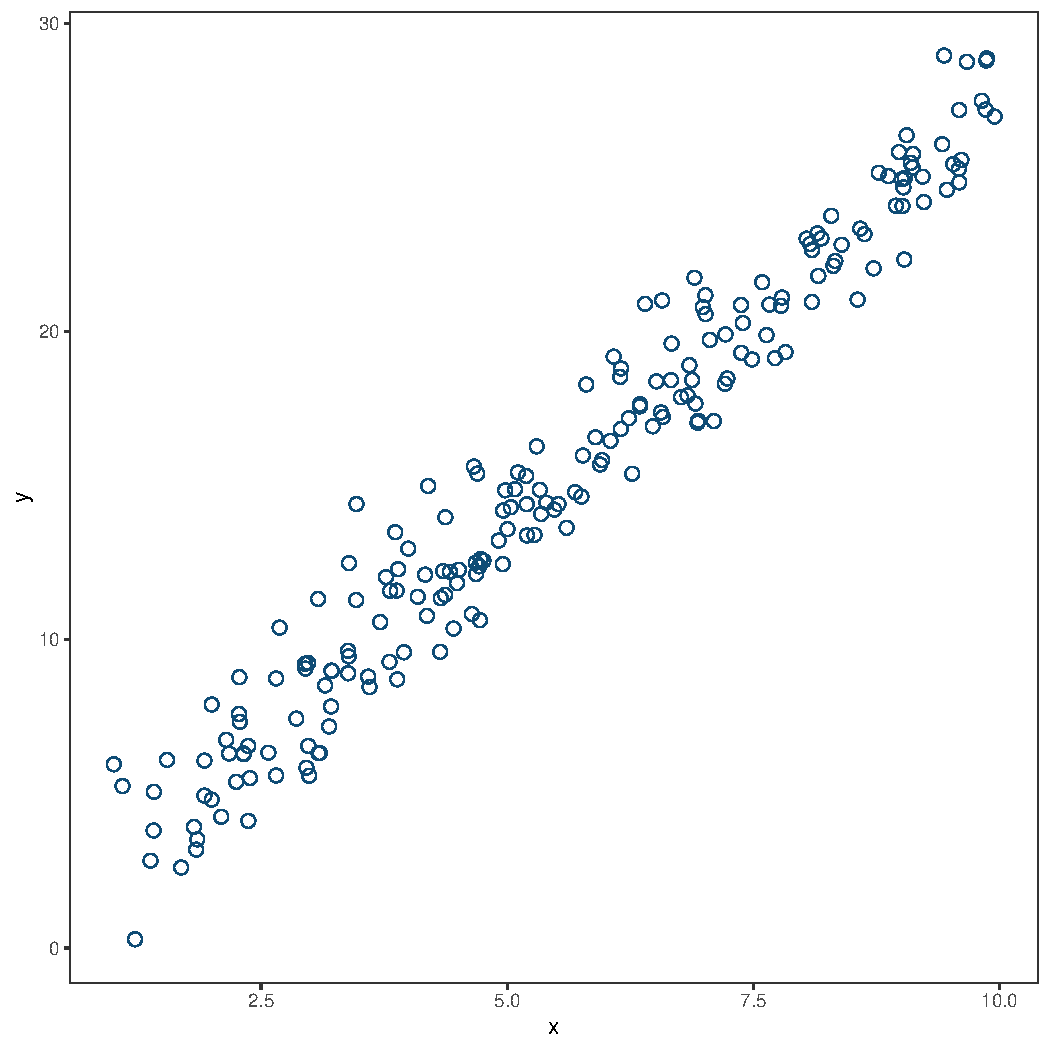
\includegraphics[scale=.5]{q2_plot1.pdf} 
	\caption{Scatter - Problem 2 data}
\end{figure}
\noindent To use Newton-Raphson algorithm in \texttt{R}, firstly define a loss function, secondly set default slope and intercept both as 0 according to the scatter, then use BFGS method in optim function. Here are codes:\\

\lstinputlisting[language=R, firstline=93,lastline=122]{PS01_answers_Chenxi.R} 

\noindent The slope and coefficient were stored in par vector in newton\_results variable, so use this code to print: \\

\lstinputlisting[language=R, firstline=124,lastline=127]{PS01_answers_Chenxi.R} 

\noindent We got the answers:
\begin{verbatim}
	In Newton-Raphson algorithm, my results are: 
	The intercept is: 0.138529 
	The slope is: 2.726599 
\end{verbatim}

\noindent To show the equivalent results with \texttt{lm}, I use these codes:\\
\lstinputlisting[language=R, firstline=129,lastline=135]{PS01_answers_Chenxi.R} 

\noindent We got the answers:
\begin{verbatim}
	In lm methods, my results are: 
	The intercept is: 0.1391874 
	The slope is: 2.726699 
\end{verbatim}
\noindent Create a table to see the differences between Newton-Raphson Algorithm and lm Methods:
\begin{center}
	\begin{tabular} { |> {\centering\arraybackslash}p{5cm} |> {\centering\arraybackslash}p{3cm} |> {\centering\arraybackslash}p{3cm} |}
		\hline
		& \textbf{Intercept} & \textbf{Slope} \\
		\hline
		\textbf{Newton-Raphson Algorithm} & 0.138529 & 2.726599 \\
		\hline
		\textbf{lm Methods} & 0.1391874 & 2.726699  \\
		\hline
	\end{tabular}
\end{center}
\noindent Compared with the Newton-Raphson Algorithm intercept ($\approx$ 0.14) and slope ($\approx$ 2.73), lm methods' intercept ($\approx$ 0.14) and slope ($\approx$ 2.73) is near the same. And we can write our regression formula like this: \\

\noindent $y = 0.14 + 2.73 x$ \\

\noindent \noindent Here is the explain of these 2 methods get the similar but not the same results:\\

\begin{itemize}
	\item  Due to differences in numerical computation precision, computational methods, and implementation details of the optimization algorithms, minor differences may arise. These differences are typically negligible and do not significantly affect the final model fitting results.\\
\end{itemize}

\end{document}
